\documentclass[twoside]{book}

% Packages required by doxygen
\usepackage{fixltx2e}
\usepackage{calc}
\usepackage{doxygen}
\usepackage[export]{adjustbox} % also loads graphicx
\usepackage{graphicx}
\usepackage[utf8]{inputenc}
\usepackage{makeidx}
\usepackage{multicol}
\usepackage{multirow}
\PassOptionsToPackage{warn}{textcomp}
\usepackage{textcomp}
\usepackage[nointegrals]{wasysym}
\usepackage[table]{xcolor}

% Font selection
\usepackage[T1]{fontenc}
\usepackage[scaled=.90]{helvet}
\usepackage{courier}
\usepackage{amssymb}
\usepackage{sectsty}
\renewcommand{\familydefault}{\sfdefault}
\allsectionsfont{%
  \fontseries{bc}\selectfont%
  \color{darkgray}%
}
\renewcommand{\DoxyLabelFont}{%
  \fontseries{bc}\selectfont%
  \color{darkgray}%
}
\newcommand{\+}{\discretionary{\mbox{\scriptsize$\hookleftarrow$}}{}{}}

% Page & text layout
\usepackage{geometry}
\geometry{%
  a4paper,%
  top=2.5cm,%
  bottom=2.5cm,%
  left=2.5cm,%
  right=2.5cm%
}
\tolerance=750
\hfuzz=15pt
\hbadness=750
\setlength{\emergencystretch}{15pt}
\setlength{\parindent}{0cm}
\setlength{\parskip}{3ex plus 2ex minus 2ex}
\makeatletter
\renewcommand{\paragraph}{%
  \@startsection{paragraph}{4}{0ex}{-1.0ex}{1.0ex}{%
    \normalfont\normalsize\bfseries\SS@parafont%
  }%
}
\renewcommand{\subparagraph}{%
  \@startsection{subparagraph}{5}{0ex}{-1.0ex}{1.0ex}{%
    \normalfont\normalsize\bfseries\SS@subparafont%
  }%
}
\makeatother

% Headers & footers
\usepackage{fancyhdr}
\pagestyle{fancyplain}
\fancyhead[LE]{\fancyplain{}{\bfseries\thepage}}
\fancyhead[CE]{\fancyplain{}{}}
\fancyhead[RE]{\fancyplain{}{\bfseries\leftmark}}
\fancyhead[LO]{\fancyplain{}{\bfseries\rightmark}}
\fancyhead[CO]{\fancyplain{}{}}
\fancyhead[RO]{\fancyplain{}{\bfseries\thepage}}
\fancyfoot[LE]{\fancyplain{}{}}
\fancyfoot[CE]{\fancyplain{}{}}
\fancyfoot[RE]{\fancyplain{}{\bfseries\scriptsize Generated by Doxygen }}
\fancyfoot[LO]{\fancyplain{}{\bfseries\scriptsize Generated by Doxygen }}
\fancyfoot[CO]{\fancyplain{}{}}
\fancyfoot[RO]{\fancyplain{}{}}
\renewcommand{\footrulewidth}{0.4pt}
\renewcommand{\chaptermark}[1]{%
  \markboth{#1}{}%
}
\renewcommand{\sectionmark}[1]{%
  \markright{\thesection\ #1}%
}

% Indices & bibliography
\usepackage{natbib}
\usepackage[titles]{tocloft}
\setcounter{tocdepth}{3}
\setcounter{secnumdepth}{5}
\makeindex

% Hyperlinks (required, but should be loaded last)
\usepackage{ifpdf}
\ifpdf
  \usepackage[pdftex,pagebackref=true]{hyperref}
\else
  \usepackage[ps2pdf,pagebackref=true]{hyperref}
\fi
\hypersetup{%
  colorlinks=true,%
  linkcolor=blue,%
  citecolor=blue,%
  unicode%
}

% Custom commands
\newcommand{\clearemptydoublepage}{%
  \newpage{\pagestyle{empty}\cleardoublepage}%
}

\usepackage{caption}
\captionsetup{labelsep=space,justification=centering,font={bf},singlelinecheck=off,skip=4pt,position=top}

%===== C O N T E N T S =====

\begin{document}

% Titlepage & ToC
\hypersetup{pageanchor=false,
             bookmarksnumbered=true,
             pdfencoding=unicode
            }
\pagenumbering{alph}
\begin{titlepage}
\vspace*{7cm}
\begin{center}%
{\Large Not\+Wordle }\\
\vspace*{1cm}
{\large Generated by Doxygen 1.8.13}\\
\end{center}
\end{titlepage}
\clearemptydoublepage
\pagenumbering{roman}
\tableofcontents
\clearemptydoublepage
\pagenumbering{arabic}
\hypersetup{pageanchor=true}

%--- Begin generated contents ---
\chapter{Main Page}
\label{index}\hypertarget{index}{}\href{https://codecov.io/gh/s-merritt/NotWordle}{\tt }

\section*{Not\+Wordle}

just a little side project of mine to recreate the game Wordle.

The game is currently just text-\/based, but I have plans to make it an Android app.

\subsection*{How to Build}

This project is currently built with C\+Make ($>$ v3.\+10) using G\+CC v7.\+5.\+0.

You can build the project by pulling the source code and running the {\ttfamily build.\+sh} script


\begin{DoxyCode}
./build.sh
\end{DoxyCode}


\subsection*{How to Run}

After calling the {\ttfamily build.\+sh} script, you can run the generated executable in the build folder like so


\begin{DoxyCode}
./build/bin/NotWordle
\end{DoxyCode}


\subsection*{How to Play}

The player is given the option for the length of the word they wish to guess. The number of guesses the player will get is equal to the length of the word plus one. The default length is 5, entering nothing will select this value.

After you have selected a word size, the game will begin. Type in a valid word of that length to enter it as a guess. The game will confirm your answer before revealing the results.

Once a guess is entered, the game will reveal the validity of each letter in your guess\+:


\begin{DoxyItemize}
\item G\+R\+E\+EN\+: the letter is in the word and in the correct place
\item B\+L\+UE\+: the letter is in the word, but in the wrong place
\item R\+ED\+: the letter is not in the word
\end{DoxyItemize}

You will also be presented with an alphabet that updates with the colors of the letters you\textquotesingle{}ve guessed. Bear in mind that some words will have multiple of the same letter!

If you guess the word before you\textquotesingle{}ve run out of guesses, you win! 
\chapter{Hierarchical Index}
\section{Class Hierarchy}
This inheritance list is sorted roughly, but not completely, alphabetically\+:\begin{DoxyCompactList}
\item \contentsline{section}{game\+:\+:Dictionary}{\pageref{classgame_1_1Dictionary}}{}
\item \contentsline{section}{game\+:\+:Game}{\pageref{classgame_1_1Game}}{}
\item \contentsline{section}{game\+:\+:objects\+:\+:Game\+Object}{\pageref{classgame_1_1objects_1_1GameObject}}{}
\begin{DoxyCompactList}
\item \contentsline{section}{game\+:\+:objects\+:\+:Grid}{\pageref{classgame_1_1objects_1_1Grid}}{}
\item \contentsline{section}{game\+:\+:objects\+:\+:Space}{\pageref{classgame_1_1objects_1_1Space}}{}
\end{DoxyCompactList}
\end{DoxyCompactList}

\chapter{Class Index}
\section{Class List}
Here are the classes, structs, unions and interfaces with brief descriptions\+:\begin{DoxyCompactList}
\item\contentsline{section}{\hyperlink{classgame_1_1Dictionary}{game\+::\+Dictionary} \\*\hyperlink{classgame_1_1Dictionary}{Dictionary} class for handling acceptable words for the game. Loads words from system file }{\pageref{classgame_1_1Dictionary}}{}
\item\contentsline{section}{\hyperlink{classgame_1_1Game}{game\+::\+Game} \\*Main class for running the actual game, handling most of the user input and output }{\pageref{classgame_1_1Game}}{}
\item\contentsline{section}{\hyperlink{classgame_1_1objects_1_1GameObject}{game\+::objects\+::\+Game\+Object} \\*Top-\/\+Level class that all objects of the game will inherit from, this is mostly for book-\/keeping }{\pageref{classgame_1_1objects_1_1GameObject}}{}
\item\contentsline{section}{\hyperlink{classgame_1_1objects_1_1Grid}{game\+::objects\+::\+Grid} \\*\hyperlink{classgame_1_1objects_1_1Grid}{Grid} class to contain 2D grid of Spaces for showing the user\textquotesingle{}s guesses as the game progresses }{\pageref{classgame_1_1objects_1_1Grid}}{}
\item\contentsline{section}{\hyperlink{classgame_1_1objects_1_1Space}{game\+::objects\+::\+Space} \\*\hyperlink{classgame_1_1objects_1_1Space}{Space} class for managing letters within the game \hyperlink{classgame_1_1objects_1_1Grid}{Grid} }{\pageref{classgame_1_1objects_1_1Space}}{}
\end{DoxyCompactList}

\chapter{File Index}
\section{File List}
Here is a list of all documented files with brief descriptions\+:\begin{DoxyCompactList}
\item\contentsline{section}{inc/game/\hyperlink{Color_8h}{Color.\+h} }{\pageref{Color_8h}}{}
\item\contentsline{section}{inc/game/\hyperlink{Dictionary_8h}{Dictionary.\+h} }{\pageref{Dictionary_8h}}{}
\item\contentsline{section}{inc/game/{\bfseries Game.\+h} }{\pageref{Game_8h}}{}
\item\contentsline{section}{inc/game/\hyperlink{Validity_8h}{Validity.\+h} }{\pageref{Validity_8h}}{}
\item\contentsline{section}{inc/game/objects/{\bfseries Game\+Object.\+h} }{\pageref{GameObject_8h}}{}
\item\contentsline{section}{inc/game/objects/{\bfseries Grid.\+h} }{\pageref{Grid_8h}}{}
\item\contentsline{section}{inc/game/objects/{\bfseries Space.\+h} }{\pageref{Space_8h}}{}
\end{DoxyCompactList}

\chapter{Class Documentation}
\hypertarget{classgame_1_1Dictionary}{}\section{game\+:\+:Dictionary Class Reference}
\label{classgame_1_1Dictionary}\index{game\+::\+Dictionary@{game\+::\+Dictionary}}


\hyperlink{classgame_1_1Dictionary}{Dictionary} class for handling acceptable words for the game. Loads words from system file.  




{\ttfamily \#include $<$Dictionary.\+h$>$}

\subsection*{Public Member Functions}
\begin{DoxyCompactItemize}
\item 
\mbox{\Hypertarget{classgame_1_1Dictionary_a89100f68c563cb86629343bdf46a0838}\label{classgame_1_1Dictionary_a89100f68c563cb86629343bdf46a0838}} 
\hyperlink{classgame_1_1Dictionary_a89100f68c563cb86629343bdf46a0838}{Dictionary} ()
\begin{DoxyCompactList}\small\item\em Construct a default \hyperlink{classgame_1_1Dictionary}{Dictionary} object. It will load all the words in the system file regardless of size. \end{DoxyCompactList}\item 
\mbox{\Hypertarget{classgame_1_1Dictionary_a2033b05d73fd3fc7f5de4722bf8cae17}\label{classgame_1_1Dictionary_a2033b05d73fd3fc7f5de4722bf8cae17}} 
void \hyperlink{classgame_1_1Dictionary_a2033b05d73fd3fc7f5de4722bf8cae17}{Load\+Words} ()
\begin{DoxyCompactList}\small\item\em Goes into the /usr/share/dict/words system file and loads them into a set. Words that are proper nouns (i.\+e. that have first letter capitalized) and words that have dashes or numbers in them are filtered out. \end{DoxyCompactList}\item 
void \hyperlink{classgame_1_1Dictionary_af2b2b73b84ba946ad6cf81251bde39f9}{Load\+Words} (const int size)
\begin{DoxyCompactList}\small\item\em Same as Load\+Words but adds the additional filter of word size. \end{DoxyCompactList}\item 
bool \hyperlink{classgame_1_1Dictionary_ab799d311640149a54645e2d1d2fd2c85}{Exists} (const std\+::string \&word) const
\begin{DoxyCompactList}\small\item\em Checks if the given word exists in the loaded dictionary. \end{DoxyCompactList}\item 
std\+::string \hyperlink{classgame_1_1Dictionary_aef5f57bd6ea644ba79c1982b8a5f5f33}{Select\+Random\+Word} (const int size) const
\begin{DoxyCompactList}\small\item\em Randomly selects a word from the set of loaded words. \end{DoxyCompactList}\item 
std\+::set$<$ std\+::string $>$ \hyperlink{classgame_1_1Dictionary_a7e0711a581d356b2106ef1a0ecbb00bf}{Get\+All\+Words} ()
\begin{DoxyCompactList}\small\item\em Get the set of words currently loaded. \end{DoxyCompactList}\end{DoxyCompactItemize}


\subsection{Detailed Description}
\hyperlink{classgame_1_1Dictionary}{Dictionary} class for handling acceptable words for the game. Loads words from system file. 

\subsection{Member Function Documentation}
\mbox{\Hypertarget{classgame_1_1Dictionary_ab799d311640149a54645e2d1d2fd2c85}\label{classgame_1_1Dictionary_ab799d311640149a54645e2d1d2fd2c85}} 
\index{game\+::\+Dictionary@{game\+::\+Dictionary}!Exists@{Exists}}
\index{Exists@{Exists}!game\+::\+Dictionary@{game\+::\+Dictionary}}
\subsubsection{\texorpdfstring{Exists()}{Exists()}}
{\footnotesize\ttfamily bool game\+::\+Dictionary\+::\+Exists (\begin{DoxyParamCaption}\item[{const std\+::string \&}]{word }\end{DoxyParamCaption}) const}



Checks if the given word exists in the loaded dictionary. 


\begin{DoxyParams}{Parameters}
{\em word} & \char`\"{}word\char`\"{} whose existence is being questioned \\
\hline
\end{DoxyParams}
\begin{DoxyReturn}{Returns}
bool true if word is found, false otherwise 
\end{DoxyReturn}
\mbox{\Hypertarget{classgame_1_1Dictionary_a7e0711a581d356b2106ef1a0ecbb00bf}\label{classgame_1_1Dictionary_a7e0711a581d356b2106ef1a0ecbb00bf}} 
\index{game\+::\+Dictionary@{game\+::\+Dictionary}!Get\+All\+Words@{Get\+All\+Words}}
\index{Get\+All\+Words@{Get\+All\+Words}!game\+::\+Dictionary@{game\+::\+Dictionary}}
\subsubsection{\texorpdfstring{Get\+All\+Words()}{GetAllWords()}}
{\footnotesize\ttfamily std\+::set$<$std\+::string$>$ game\+::\+Dictionary\+::\+Get\+All\+Words (\begin{DoxyParamCaption}{ }\end{DoxyParamCaption})}



Get the set of words currently loaded. 

\begin{DoxyReturn}{Returns}
std\+::set$<$std\+::string$>$ containing loaded words 
\end{DoxyReturn}
\mbox{\Hypertarget{classgame_1_1Dictionary_af2b2b73b84ba946ad6cf81251bde39f9}\label{classgame_1_1Dictionary_af2b2b73b84ba946ad6cf81251bde39f9}} 
\index{game\+::\+Dictionary@{game\+::\+Dictionary}!Load\+Words@{Load\+Words}}
\index{Load\+Words@{Load\+Words}!game\+::\+Dictionary@{game\+::\+Dictionary}}
\subsubsection{\texorpdfstring{Load\+Words()}{LoadWords()}}
{\footnotesize\ttfamily void game\+::\+Dictionary\+::\+Load\+Words (\begin{DoxyParamCaption}\item[{const int}]{size }\end{DoxyParamCaption})}



Same as Load\+Words but adds the additional filter of word size. 


\begin{DoxyParams}{Parameters}
{\em size} & expected size of all words being loaded \\
\hline
\end{DoxyParams}
\mbox{\Hypertarget{classgame_1_1Dictionary_aef5f57bd6ea644ba79c1982b8a5f5f33}\label{classgame_1_1Dictionary_aef5f57bd6ea644ba79c1982b8a5f5f33}} 
\index{game\+::\+Dictionary@{game\+::\+Dictionary}!Select\+Random\+Word@{Select\+Random\+Word}}
\index{Select\+Random\+Word@{Select\+Random\+Word}!game\+::\+Dictionary@{game\+::\+Dictionary}}
\subsubsection{\texorpdfstring{Select\+Random\+Word()}{SelectRandomWord()}}
{\footnotesize\ttfamily std\+::string game\+::\+Dictionary\+::\+Select\+Random\+Word (\begin{DoxyParamCaption}\item[{const int}]{size }\end{DoxyParamCaption}) const}



Randomly selects a word from the set of loaded words. 


\begin{DoxyParams}{Parameters}
{\em size} & size of the random word \\
\hline
\end{DoxyParams}
\begin{DoxyReturn}{Returns}
std\+::string a random word from the set of loaded words 
\end{DoxyReturn}


The documentation for this class was generated from the following file\+:\begin{DoxyCompactItemize}
\item 
inc/game/\hyperlink{Dictionary_8h}{Dictionary.\+h}\end{DoxyCompactItemize}

\hypertarget{classgame_1_1Game}{}\section{game\+:\+:Game Class Reference}
\label{classgame_1_1Game}\index{game\+::\+Game@{game\+::\+Game}}


main class for running the actual game, handling most of the user input and output.  




{\ttfamily \#include $<$Game.\+h$>$}

\subsection*{Public Member Functions}
\begin{DoxyCompactItemize}
\item 
\mbox{\Hypertarget{classgame_1_1Game_a74cd9697144c5bb5ccf1d2cb71d56e41}\label{classgame_1_1Game_a74cd9697144c5bb5ccf1d2cb71d56e41}} 
\hyperlink{classgame_1_1Game_a74cd9697144c5bb5ccf1d2cb71d56e41}{Game} ()
\begin{DoxyCompactList}\small\item\em Construct a new \hyperlink{classgame_1_1Game}{Game} object. Initializes the array of available letters. \end{DoxyCompactList}\item 
void \hyperlink{classgame_1_1Game_afbb584718c566dd27f6e2d8fe0085d8c}{Run} (std\+::ostream \&out, std\+::istream \&in, std\+::string preselected=\char`\"{}\char`\"{})
\begin{DoxyCompactList}\small\item\em main runner function that contains the game code \end{DoxyCompactList}\item 
std\+::string \hyperlink{classgame_1_1Game_a4a16bdf4073caea5efc9c4b70b1b969f}{Query\+User\+For\+Guess} (std\+::ostream \&out, std\+::istream \&in)
\begin{DoxyCompactList}\small\item\em asks the user for a guess, including checks for invalid words \end{DoxyCompactList}\item 
uint16\+\_\+t \hyperlink{classgame_1_1Game_a3352c8a498b17b0a374d4a696fc2abdf}{Query\+User\+For\+Word\+Size} (std\+::ostream \&out, std\+::istream \&in)
\begin{DoxyCompactList}\small\item\em asks the user for the desired word size for the game, including error checking for invalid answers. Size must be between 4 and 9 \end{DoxyCompactList}\item 
bool \hyperlink{classgame_1_1Game_a729991a58de1542bdda32a0cc2778899}{Is\+Valid\+Word} (const std\+::string \&word)
\begin{DoxyCompactList}\small\item\em checks the \hyperlink{classgame_1_1Dictionary}{Dictionary} if the given word is valid \end{DoxyCompactList}\item 
void \hyperlink{classgame_1_1Game_aa86e27688c8e1d513c47afc53467dbea}{Print\+Grid} (std\+::ostream \&out)
\begin{DoxyCompactList}\small\item\em prints the Grid Spaces in a format based on the word size. \end{DoxyCompactList}\item 
void \hyperlink{classgame_1_1Game_a156ae4dc99b8adb87a83d2c72ab24285}{Show\+Available\+Letters} (std\+::ostream \&out)
\begin{DoxyCompactList}\small\item\em prints out the list of letters based on their set Validity \end{DoxyCompactList}\item 
const std\+::array$<$ \hyperlink{Validity_8h_acb8ce664e8a953fe8c27d7f0b37cbca4}{Validity}, 26 $>$ \& \hyperlink{classgame_1_1Game_aa2b90ae6940730e872300d2727a86f24}{Available\+Letters} ()
\begin{DoxyCompactList}\small\item\em getter for the validity list (index corresponds to letter in alphabet) \end{DoxyCompactList}\item 
\hyperlink{classgame_1_1Dictionary}{Dictionary} \& \hyperlink{classgame_1_1Game_a59a7ae6a629f360d6aa7c9b74a33125b}{Get\+Dictionary} ()
\begin{DoxyCompactList}\small\item\em Get the \hyperlink{classgame_1_1Dictionary}{Dictionary} object. \end{DoxyCompactList}\item 
void \hyperlink{classgame_1_1Game_a92368c63688b94a1b67f7fefb3449e9e}{Initialize\+Grid} (const int size)
\begin{DoxyCompactList}\small\item\em re-\/initializes the Grid object to the given size \end{DoxyCompactList}\item 
void \hyperlink{classgame_1_1Game_a7785bad3273c5c3be55ad44fbe78b117}{Update\+Grid} (const std\+::string \&word)
\begin{DoxyCompactList}\small\item\em updates the grid with the given word \end{DoxyCompactList}\item 
bool \hyperlink{classgame_1_1Game_a73e4f12d9ffbf48573d3e9871a15fd8e}{Check\+Guess} (const std\+::string \&game\+\_\+word)
\begin{DoxyCompactList}\small\item\em checks if the latest guess in the Grid matches the given game word. \end{DoxyCompactList}\item 
const std\+::string \& \hyperlink{classgame_1_1Game_a85584931f1e9085bd8cad92d43fd2be8}{Selected\+Word} ()
\begin{DoxyCompactList}\small\item\em returns the selected word of the game \end{DoxyCompactList}\end{DoxyCompactItemize}


\subsection{Detailed Description}
main class for running the actual game, handling most of the user input and output. 

\subsection{Member Function Documentation}
\mbox{\Hypertarget{classgame_1_1Game_aa2b90ae6940730e872300d2727a86f24}\label{classgame_1_1Game_aa2b90ae6940730e872300d2727a86f24}} 
\index{game\+::\+Game@{game\+::\+Game}!Available\+Letters@{Available\+Letters}}
\index{Available\+Letters@{Available\+Letters}!game\+::\+Game@{game\+::\+Game}}
\subsubsection{\texorpdfstring{Available\+Letters()}{AvailableLetters()}}
{\footnotesize\ttfamily const std\+::array$<$\hyperlink{Validity_8h_acb8ce664e8a953fe8c27d7f0b37cbca4}{Validity}, 26$>$\& game\+::\+Game\+::\+Available\+Letters (\begin{DoxyParamCaption}{ }\end{DoxyParamCaption})}



getter for the validity list (index corresponds to letter in alphabet) 

\begin{DoxyReturn}{Returns}
const std\+::array$<$\+Validity, 26$>$\& 
\end{DoxyReturn}
\mbox{\Hypertarget{classgame_1_1Game_a73e4f12d9ffbf48573d3e9871a15fd8e}\label{classgame_1_1Game_a73e4f12d9ffbf48573d3e9871a15fd8e}} 
\index{game\+::\+Game@{game\+::\+Game}!Check\+Guess@{Check\+Guess}}
\index{Check\+Guess@{Check\+Guess}!game\+::\+Game@{game\+::\+Game}}
\subsubsection{\texorpdfstring{Check\+Guess()}{CheckGuess()}}
{\footnotesize\ttfamily bool game\+::\+Game\+::\+Check\+Guess (\begin{DoxyParamCaption}\item[{const std\+::string \&}]{game\+\_\+word }\end{DoxyParamCaption})}



checks if the latest guess in the Grid matches the given game word. 


\begin{DoxyParams}{Parameters}
{\em game\+\_\+word} & selected word for the game \\
\hline
\end{DoxyParams}
\begin{DoxyReturn}{Returns}
bool true if the words match, false otherwise 
\end{DoxyReturn}
\mbox{\Hypertarget{classgame_1_1Game_a59a7ae6a629f360d6aa7c9b74a33125b}\label{classgame_1_1Game_a59a7ae6a629f360d6aa7c9b74a33125b}} 
\index{game\+::\+Game@{game\+::\+Game}!Get\+Dictionary@{Get\+Dictionary}}
\index{Get\+Dictionary@{Get\+Dictionary}!game\+::\+Game@{game\+::\+Game}}
\subsubsection{\texorpdfstring{Get\+Dictionary()}{GetDictionary()}}
{\footnotesize\ttfamily \hyperlink{classgame_1_1Dictionary}{Dictionary}\& game\+::\+Game\+::\+Get\+Dictionary (\begin{DoxyParamCaption}{ }\end{DoxyParamCaption})}



Get the \hyperlink{classgame_1_1Dictionary}{Dictionary} object. 

\begin{DoxyReturn}{Returns}
\hyperlink{classgame_1_1Dictionary}{Dictionary}\& 
\end{DoxyReturn}
\mbox{\Hypertarget{classgame_1_1Game_a92368c63688b94a1b67f7fefb3449e9e}\label{classgame_1_1Game_a92368c63688b94a1b67f7fefb3449e9e}} 
\index{game\+::\+Game@{game\+::\+Game}!Initialize\+Grid@{Initialize\+Grid}}
\index{Initialize\+Grid@{Initialize\+Grid}!game\+::\+Game@{game\+::\+Game}}
\subsubsection{\texorpdfstring{Initialize\+Grid()}{InitializeGrid()}}
{\footnotesize\ttfamily void game\+::\+Game\+::\+Initialize\+Grid (\begin{DoxyParamCaption}\item[{const int}]{size }\end{DoxyParamCaption})}



re-\/initializes the Grid object to the given size 


\begin{DoxyParams}{Parameters}
{\em size} & size of the grid \\
\hline
\end{DoxyParams}
\mbox{\Hypertarget{classgame_1_1Game_a729991a58de1542bdda32a0cc2778899}\label{classgame_1_1Game_a729991a58de1542bdda32a0cc2778899}} 
\index{game\+::\+Game@{game\+::\+Game}!Is\+Valid\+Word@{Is\+Valid\+Word}}
\index{Is\+Valid\+Word@{Is\+Valid\+Word}!game\+::\+Game@{game\+::\+Game}}
\subsubsection{\texorpdfstring{Is\+Valid\+Word()}{IsValidWord()}}
{\footnotesize\ttfamily bool game\+::\+Game\+::\+Is\+Valid\+Word (\begin{DoxyParamCaption}\item[{const std\+::string \&}]{word }\end{DoxyParamCaption})}



checks the \hyperlink{classgame_1_1Dictionary}{Dictionary} if the given word is valid 


\begin{DoxyParams}{Parameters}
{\em word} & word being checked \\
\hline
\end{DoxyParams}
\begin{DoxyReturn}{Returns}
bool true if word is in \hyperlink{classgame_1_1Dictionary}{Dictionary}, false otherwise 
\end{DoxyReturn}
\mbox{\Hypertarget{classgame_1_1Game_aa86e27688c8e1d513c47afc53467dbea}\label{classgame_1_1Game_aa86e27688c8e1d513c47afc53467dbea}} 
\index{game\+::\+Game@{game\+::\+Game}!Print\+Grid@{Print\+Grid}}
\index{Print\+Grid@{Print\+Grid}!game\+::\+Game@{game\+::\+Game}}
\subsubsection{\texorpdfstring{Print\+Grid()}{PrintGrid()}}
{\footnotesize\ttfamily void game\+::\+Game\+::\+Print\+Grid (\begin{DoxyParamCaption}\item[{std\+::ostream \&}]{out }\end{DoxyParamCaption})}



prints the Grid Spaces in a format based on the word size. 


\begin{DoxyParams}{Parameters}
{\em out} & output stream \\
\hline
\end{DoxyParams}
\mbox{\Hypertarget{classgame_1_1Game_a4a16bdf4073caea5efc9c4b70b1b969f}\label{classgame_1_1Game_a4a16bdf4073caea5efc9c4b70b1b969f}} 
\index{game\+::\+Game@{game\+::\+Game}!Query\+User\+For\+Guess@{Query\+User\+For\+Guess}}
\index{Query\+User\+For\+Guess@{Query\+User\+For\+Guess}!game\+::\+Game@{game\+::\+Game}}
\subsubsection{\texorpdfstring{Query\+User\+For\+Guess()}{QueryUserForGuess()}}
{\footnotesize\ttfamily std\+::string game\+::\+Game\+::\+Query\+User\+For\+Guess (\begin{DoxyParamCaption}\item[{std\+::ostream \&}]{out,  }\item[{std\+::istream \&}]{in }\end{DoxyParamCaption})}



asks the user for a guess, including checks for invalid words 


\begin{DoxyParams}{Parameters}
{\em out} & output stream \\
\hline
{\em in} & input stream \\
\hline
\end{DoxyParams}
\begin{DoxyReturn}{Returns}
std\+::string the final guess of the user (after error checking) 
\end{DoxyReturn}
\mbox{\Hypertarget{classgame_1_1Game_a3352c8a498b17b0a374d4a696fc2abdf}\label{classgame_1_1Game_a3352c8a498b17b0a374d4a696fc2abdf}} 
\index{game\+::\+Game@{game\+::\+Game}!Query\+User\+For\+Word\+Size@{Query\+User\+For\+Word\+Size}}
\index{Query\+User\+For\+Word\+Size@{Query\+User\+For\+Word\+Size}!game\+::\+Game@{game\+::\+Game}}
\subsubsection{\texorpdfstring{Query\+User\+For\+Word\+Size()}{QueryUserForWordSize()}}
{\footnotesize\ttfamily uint16\+\_\+t game\+::\+Game\+::\+Query\+User\+For\+Word\+Size (\begin{DoxyParamCaption}\item[{std\+::ostream \&}]{out,  }\item[{std\+::istream \&}]{in }\end{DoxyParamCaption})}



asks the user for the desired word size for the game, including error checking for invalid answers. Size must be between 4 and 9 


\begin{DoxyParams}{Parameters}
{\em out} & output stream \\
\hline
{\em in} & input stream \\
\hline
\end{DoxyParams}
\begin{DoxyReturn}{Returns}
uint16\+\_\+t the final word size from the user (after error checking) 
\end{DoxyReturn}
\mbox{\Hypertarget{classgame_1_1Game_afbb584718c566dd27f6e2d8fe0085d8c}\label{classgame_1_1Game_afbb584718c566dd27f6e2d8fe0085d8c}} 
\index{game\+::\+Game@{game\+::\+Game}!Run@{Run}}
\index{Run@{Run}!game\+::\+Game@{game\+::\+Game}}
\subsubsection{\texorpdfstring{Run()}{Run()}}
{\footnotesize\ttfamily void game\+::\+Game\+::\+Run (\begin{DoxyParamCaption}\item[{std\+::ostream \&}]{out,  }\item[{std\+::istream \&}]{in,  }\item[{std\+::string}]{preselected = {\ttfamily \char`\"{}\char`\"{}} }\end{DoxyParamCaption})}



main runner function that contains the game code 


\begin{DoxyParams}{Parameters}
{\em out} & output stream \\
\hline
{\em in} & input stream \\
\hline
{\em preselected} & for unit testing, sets the game word to this word instead of randomly selected it \\
\hline
\end{DoxyParams}
\mbox{\Hypertarget{classgame_1_1Game_a85584931f1e9085bd8cad92d43fd2be8}\label{classgame_1_1Game_a85584931f1e9085bd8cad92d43fd2be8}} 
\index{game\+::\+Game@{game\+::\+Game}!Selected\+Word@{Selected\+Word}}
\index{Selected\+Word@{Selected\+Word}!game\+::\+Game@{game\+::\+Game}}
\subsubsection{\texorpdfstring{Selected\+Word()}{SelectedWord()}}
{\footnotesize\ttfamily const std\+::string\& game\+::\+Game\+::\+Selected\+Word (\begin{DoxyParamCaption}{ }\end{DoxyParamCaption})}



returns the selected word of the game 

\begin{DoxyReturn}{Returns}
const std\+::string\& game word 
\end{DoxyReturn}
\mbox{\Hypertarget{classgame_1_1Game_a156ae4dc99b8adb87a83d2c72ab24285}\label{classgame_1_1Game_a156ae4dc99b8adb87a83d2c72ab24285}} 
\index{game\+::\+Game@{game\+::\+Game}!Show\+Available\+Letters@{Show\+Available\+Letters}}
\index{Show\+Available\+Letters@{Show\+Available\+Letters}!game\+::\+Game@{game\+::\+Game}}
\subsubsection{\texorpdfstring{Show\+Available\+Letters()}{ShowAvailableLetters()}}
{\footnotesize\ttfamily void game\+::\+Game\+::\+Show\+Available\+Letters (\begin{DoxyParamCaption}\item[{std\+::ostream \&}]{out }\end{DoxyParamCaption})}



prints out the list of letters based on their set Validity 


\begin{DoxyParams}{Parameters}
{\em out} & output stream \\
\hline
\end{DoxyParams}
\mbox{\Hypertarget{classgame_1_1Game_a7785bad3273c5c3be55ad44fbe78b117}\label{classgame_1_1Game_a7785bad3273c5c3be55ad44fbe78b117}} 
\index{game\+::\+Game@{game\+::\+Game}!Update\+Grid@{Update\+Grid}}
\index{Update\+Grid@{Update\+Grid}!game\+::\+Game@{game\+::\+Game}}
\subsubsection{\texorpdfstring{Update\+Grid()}{UpdateGrid()}}
{\footnotesize\ttfamily void game\+::\+Game\+::\+Update\+Grid (\begin{DoxyParamCaption}\item[{const std\+::string \&}]{word }\end{DoxyParamCaption})}



updates the grid with the given word 


\begin{DoxyParams}{Parameters}
{\em word} & word to be placed into the grid \\
\hline
\end{DoxyParams}


The documentation for this class was generated from the following file\+:\begin{DoxyCompactItemize}
\item 
inc/game/Game.\+h\end{DoxyCompactItemize}

\hypertarget{classgame_1_1objects_1_1GameObject}{}\section{game\+:\+:objects\+:\+:Game\+Object Class Reference}
\label{classgame_1_1objects_1_1GameObject}\index{game\+::objects\+::\+Game\+Object@{game\+::objects\+::\+Game\+Object}}


Top-\/\+Level class that all objects of the game will inherit from, this is mostly for book-\/keeping.  




{\ttfamily \#include $<$Game\+Object.\+h$>$}



Inheritance diagram for game\+:\+:objects\+:\+:Game\+Object\+:\nopagebreak
\begin{figure}[H]
\begin{center}
\leavevmode
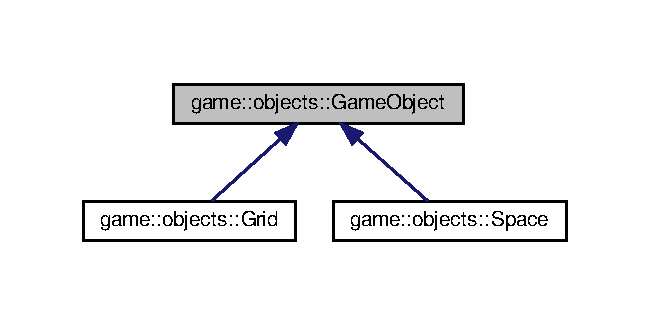
\includegraphics[width=312pt]{classgame_1_1objects_1_1GameObject__inherit__graph}
\end{center}
\end{figure}
\subsection*{Public Member Functions}
\begin{DoxyCompactItemize}
\item 
\mbox{\Hypertarget{classgame_1_1objects_1_1GameObject_abc967efcbc66ec93c8592ad785aeb953}\label{classgame_1_1objects_1_1GameObject_abc967efcbc66ec93c8592ad785aeb953}} 
virtual std\+::string \hyperlink{classgame_1_1objects_1_1GameObject_abc967efcbc66ec93c8592ad785aeb953}{Name} ()=0
\begin{DoxyCompactList}\small\item\em pure-\/virtual function for naming the object \end{DoxyCompactList}\item 
\mbox{\Hypertarget{classgame_1_1objects_1_1GameObject_a59faf4c33c2c0d8a9d52a26029d1488f}\label{classgame_1_1objects_1_1GameObject_a59faf4c33c2c0d8a9d52a26029d1488f}} 
virtual std\+::string \hyperlink{classgame_1_1objects_1_1GameObject_a59faf4c33c2c0d8a9d52a26029d1488f}{to\+\_\+string} ()=0
\begin{DoxyCompactList}\small\item\em pure-\/virtual function for converting the object to a printable string \end{DoxyCompactList}\item 
\mbox{\Hypertarget{classgame_1_1objects_1_1GameObject_a52cb48890e7b64e25ebb1fb87ddd3551}\label{classgame_1_1objects_1_1GameObject_a52cb48890e7b64e25ebb1fb87ddd3551}} 
\hyperlink{classgame_1_1objects_1_1GameObject_a52cb48890e7b64e25ebb1fb87ddd3551}{Game\+Object} ()
\begin{DoxyCompactList}\small\item\em Construct a new \hyperlink{classgame_1_1objects_1_1GameObject}{Game\+Object}. Also establishes the ID of the object. \end{DoxyCompactList}\item 
uint32\+\_\+t \hyperlink{classgame_1_1objects_1_1GameObject_a1fb35a5a82dee7aefe112b81bda8b2c4}{Get\+ID} ()
\begin{DoxyCompactList}\small\item\em Getter for the ID of the object. \end{DoxyCompactList}\end{DoxyCompactItemize}


\subsection{Detailed Description}
Top-\/\+Level class that all objects of the game will inherit from, this is mostly for book-\/keeping. 

\subsection{Member Function Documentation}
\mbox{\Hypertarget{classgame_1_1objects_1_1GameObject_a1fb35a5a82dee7aefe112b81bda8b2c4}\label{classgame_1_1objects_1_1GameObject_a1fb35a5a82dee7aefe112b81bda8b2c4}} 
\index{game\+::objects\+::\+Game\+Object@{game\+::objects\+::\+Game\+Object}!Get\+ID@{Get\+ID}}
\index{Get\+ID@{Get\+ID}!game\+::objects\+::\+Game\+Object@{game\+::objects\+::\+Game\+Object}}
\subsubsection{\texorpdfstring{Get\+I\+D()}{GetID()}}
{\footnotesize\ttfamily uint32\+\_\+t game\+::objects\+::\+Game\+Object\+::\+Get\+ID (\begin{DoxyParamCaption}{ }\end{DoxyParamCaption})\hspace{0.3cm}{\ttfamily [inline]}}



Getter for the ID of the object. 

\begin{DoxyReturn}{Returns}
uint32\+\_\+t ID 
\end{DoxyReturn}


The documentation for this class was generated from the following file\+:\begin{DoxyCompactItemize}
\item 
inc/game/objects/Game\+Object.\+h\end{DoxyCompactItemize}

\hypertarget{classgame_1_1objects_1_1Grid}{}\section{game\+:\+:objects\+:\+:Grid Class Reference}
\label{classgame_1_1objects_1_1Grid}\index{game\+::objects\+::\+Grid@{game\+::objects\+::\+Grid}}


\hyperlink{classgame_1_1objects_1_1Grid}{Grid} class to contain 2D grid of Spaces for showing the user\textquotesingle{}s guesses as the game progresses.  




{\ttfamily \#include $<$Grid.\+h$>$}



Inheritance diagram for game\+:\+:objects\+:\+:Grid\+:
\nopagebreak
\begin{figure}[H]
\begin{center}
\leavevmode
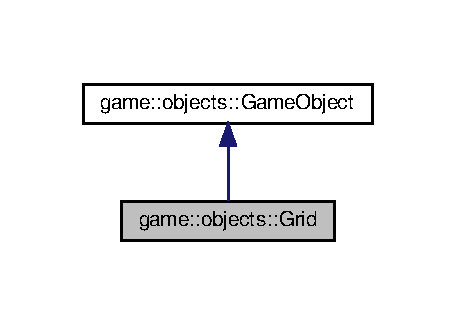
\includegraphics[width=219pt]{classgame_1_1objects_1_1Grid__inherit__graph}
\end{center}
\end{figure}


Collaboration diagram for game\+:\+:objects\+:\+:Grid\+:
\nopagebreak
\begin{figure}[H]
\begin{center}
\leavevmode
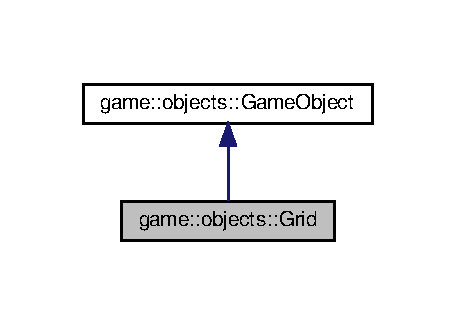
\includegraphics[width=219pt]{classgame_1_1objects_1_1Grid__coll__graph}
\end{center}
\end{figure}
\subsection*{Public Member Functions}
\begin{DoxyCompactItemize}
\item 
\mbox{\Hypertarget{classgame_1_1objects_1_1Grid_adccb0e5dcc469737ee2ed80ee0a2f69c}\label{classgame_1_1objects_1_1Grid_adccb0e5dcc469737ee2ed80ee0a2f69c}} 
\hyperlink{classgame_1_1objects_1_1Grid_adccb0e5dcc469737ee2ed80ee0a2f69c}{Grid} ()=delete
\begin{DoxyCompactList}\small\item\em delete default constructor \end{DoxyCompactList}\item 
\hyperlink{classgame_1_1objects_1_1Grid_a8ccdcfad249ef402977c9a9582ef02f7}{Grid} (int word\+\_\+size)
\begin{DoxyCompactList}\small\item\em Construct a new \hyperlink{classgame_1_1objects_1_1Grid}{Grid} object with the given word size Word size determines the number of columns, while the number of rows is word\+\_\+size + 1. \end{DoxyCompactList}\item 
\mbox{\Hypertarget{classgame_1_1objects_1_1Grid_a631c3b3217e25366b41746c3507c392f}\label{classgame_1_1objects_1_1Grid_a631c3b3217e25366b41746c3507c392f}} 
\hyperlink{classgame_1_1objects_1_1Grid_a631c3b3217e25366b41746c3507c392f}{$\sim$\+Grid} ()
\begin{DoxyCompactList}\small\item\em Destroy the \hyperlink{classgame_1_1objects_1_1Grid}{Grid} object (free up \hyperlink{classgame_1_1objects_1_1Space}{Space} memory) \end{DoxyCompactList}\item 
void \hyperlink{classgame_1_1objects_1_1Grid_ac1be0e2e0ae78559eb9581f6ea21da57}{Update\+Space} (int row, int col, char c)
\begin{DoxyCompactList}\small\item\em Updates the space at row, col with the given character. \end{DoxyCompactList}\item 
void \hyperlink{classgame_1_1objects_1_1Grid_a4ac6a9c2fcd4fac310ff3ebbe02eb56d}{Update\+Line} (const std\+::string \&word)
\begin{DoxyCompactList}\small\item\em Updates a row on the grid with the given word. Which row being updated is determined by number of guesses. \end{DoxyCompactList}\item 
\mbox{\Hypertarget{classgame_1_1objects_1_1Grid_ab5a78b3a32367cb685d4dcb501756d14}\label{classgame_1_1objects_1_1Grid_ab5a78b3a32367cb685d4dcb501756d14}} 
void \hyperlink{classgame_1_1objects_1_1Grid_ab5a78b3a32367cb685d4dcb501756d14}{Clear\+Line} ()
\begin{DoxyCompactList}\small\item\em Clears a row on the grid, resetting each \hyperlink{classgame_1_1objects_1_1Space}{Space}. Which row being updated is determined by number of guesses. \end{DoxyCompactList}\item 
bool \hyperlink{classgame_1_1objects_1_1Grid_ad1cd48d90e6886a6bde6b1905319d8e5}{Check\+Guess} (const std\+::string \&exp\+\_\+word)
\begin{DoxyCompactList}\small\item\em Checks if the current guess matches the given word. The current guess is whatever word is in the last row (based on number of guesses) \end{DoxyCompactList}\item 
bool \hyperlink{classgame_1_1objects_1_1Grid_a8074b85524ccdff89f5a520699599f32}{Increment\+Guess} ()
\begin{DoxyCompactList}\small\item\em increments the number of guesses field and checks if that field is greater than the number of rows (i.\+e. game over) \end{DoxyCompactList}\item 
std\+::size\+\_\+t \hyperlink{classgame_1_1objects_1_1Grid_ad6a36b9043e9e5b5318149a9c7908933}{Index} (int row, int col) const
\begin{DoxyCompactList}\small\item\em Helper function to get the row-\/major index for (row, col) in vectorized grid. \end{DoxyCompactList}\item 
std\+::string \hyperlink{classgame_1_1objects_1_1Grid_af54fe43e853745e264a5b9e9b9e8e702}{Get\+Current\+Guess} ()
\begin{DoxyCompactList}\small\item\em Gets the latest guess entered into the grid. \end{DoxyCompactList}\item 
\hyperlink{classgame_1_1objects_1_1Space}{Space} \& \hyperlink{classgame_1_1objects_1_1Grid_a90aff1cebba7fa8de3d5dd452d59364c}{Get\+Space} (int row, int col)
\begin{DoxyCompactList}\small\item\em Get the \hyperlink{classgame_1_1objects_1_1Space}{Space} located at (row, col) in the grid. \end{DoxyCompactList}\item 
void \hyperlink{classgame_1_1objects_1_1Grid_aba01074c988b3732d7de432c5dd558ac}{Mark\+Letters\+Used} (std\+::array$<$ \hyperlink{Validity_8h_acb8ce664e8a953fe8c27d7f0b37cbca4}{Validity}, 26 $>$ $\ast$alphabet)
\begin{DoxyCompactList}\small\item\em Checks the grid for which letters have been used; it will examine the Validity at each \hyperlink{classgame_1_1objects_1_1Space}{Space} and mark it accordingly in the given Validity array. \end{DoxyCompactList}\item 
std\+::string \hyperlink{classgame_1_1objects_1_1Grid_a1a10441dea475af11c796995af6e9855}{Name} () override
\begin{DoxyCompactList}\small\item\em Gets the Name of the object. \end{DoxyCompactList}\item 
std\+::string \hyperlink{classgame_1_1objects_1_1Grid_a3ecc419e20319a116b0a467e064e0403}{to\+\_\+string} () override
\begin{DoxyCompactList}\small\item\em Converts the grid to a human-\/readable grid of Spaces. \end{DoxyCompactList}\item 
std\+::pair$<$ const int, const int $>$ \hyperlink{classgame_1_1objects_1_1Grid_a16bf69070bed5732b1a42a97b83ea2cb}{Get\+Grid\+Dimensions} () const
\begin{DoxyCompactList}\small\item\em Getter for the dimensions of the grid. \end{DoxyCompactList}\end{DoxyCompactItemize}


\subsection{Detailed Description}
\hyperlink{classgame_1_1objects_1_1Grid}{Grid} class to contain 2D grid of Spaces for showing the user\textquotesingle{}s guesses as the game progresses. 

\subsection{Constructor \& Destructor Documentation}
\mbox{\Hypertarget{classgame_1_1objects_1_1Grid_a8ccdcfad249ef402977c9a9582ef02f7}\label{classgame_1_1objects_1_1Grid_a8ccdcfad249ef402977c9a9582ef02f7}} 
\index{game\+::objects\+::\+Grid@{game\+::objects\+::\+Grid}!Grid@{Grid}}
\index{Grid@{Grid}!game\+::objects\+::\+Grid@{game\+::objects\+::\+Grid}}
\subsubsection{\texorpdfstring{Grid()}{Grid()}}
{\footnotesize\ttfamily game\+::objects\+::\+Grid\+::\+Grid (\begin{DoxyParamCaption}\item[{int}]{word\+\_\+size }\end{DoxyParamCaption})}



Construct a new \hyperlink{classgame_1_1objects_1_1Grid}{Grid} object with the given word size Word size determines the number of columns, while the number of rows is word\+\_\+size + 1. 


\begin{DoxyParams}{Parameters}
{\em word\+\_\+size} & word size of the grim (and number of columns) \\
\hline
\end{DoxyParams}


\subsection{Member Function Documentation}
\mbox{\Hypertarget{classgame_1_1objects_1_1Grid_ad1cd48d90e6886a6bde6b1905319d8e5}\label{classgame_1_1objects_1_1Grid_ad1cd48d90e6886a6bde6b1905319d8e5}} 
\index{game\+::objects\+::\+Grid@{game\+::objects\+::\+Grid}!Check\+Guess@{Check\+Guess}}
\index{Check\+Guess@{Check\+Guess}!game\+::objects\+::\+Grid@{game\+::objects\+::\+Grid}}
\subsubsection{\texorpdfstring{Check\+Guess()}{CheckGuess()}}
{\footnotesize\ttfamily bool game\+::objects\+::\+Grid\+::\+Check\+Guess (\begin{DoxyParamCaption}\item[{const std\+::string \&}]{exp\+\_\+word }\end{DoxyParamCaption})}



Checks if the current guess matches the given word. The current guess is whatever word is in the last row (based on number of guesses) 


\begin{DoxyParams}{Parameters}
{\em exp\+\_\+word} & \\
\hline
\end{DoxyParams}
\begin{DoxyReturn}{Returns}
true if words match, false otherwise 
\end{DoxyReturn}
\mbox{\Hypertarget{classgame_1_1objects_1_1Grid_af54fe43e853745e264a5b9e9b9e8e702}\label{classgame_1_1objects_1_1Grid_af54fe43e853745e264a5b9e9b9e8e702}} 
\index{game\+::objects\+::\+Grid@{game\+::objects\+::\+Grid}!Get\+Current\+Guess@{Get\+Current\+Guess}}
\index{Get\+Current\+Guess@{Get\+Current\+Guess}!game\+::objects\+::\+Grid@{game\+::objects\+::\+Grid}}
\subsubsection{\texorpdfstring{Get\+Current\+Guess()}{GetCurrentGuess()}}
{\footnotesize\ttfamily std\+::string game\+::objects\+::\+Grid\+::\+Get\+Current\+Guess (\begin{DoxyParamCaption}{ }\end{DoxyParamCaption})}



Gets the latest guess entered into the grid. 

\begin{DoxyReturn}{Returns}
std\+::string latest guess 
\end{DoxyReturn}
\mbox{\Hypertarget{classgame_1_1objects_1_1Grid_a16bf69070bed5732b1a42a97b83ea2cb}\label{classgame_1_1objects_1_1Grid_a16bf69070bed5732b1a42a97b83ea2cb}} 
\index{game\+::objects\+::\+Grid@{game\+::objects\+::\+Grid}!Get\+Grid\+Dimensions@{Get\+Grid\+Dimensions}}
\index{Get\+Grid\+Dimensions@{Get\+Grid\+Dimensions}!game\+::objects\+::\+Grid@{game\+::objects\+::\+Grid}}
\subsubsection{\texorpdfstring{Get\+Grid\+Dimensions()}{GetGridDimensions()}}
{\footnotesize\ttfamily std\+::pair$<$const int, const int$>$ game\+::objects\+::\+Grid\+::\+Get\+Grid\+Dimensions (\begin{DoxyParamCaption}{ }\end{DoxyParamCaption}) const}



Getter for the dimensions of the grid. 

\begin{DoxyReturn}{Returns}
std\+::pair$<$const int, const int$>$ (num rows, num columns) 
\end{DoxyReturn}
\mbox{\Hypertarget{classgame_1_1objects_1_1Grid_a90aff1cebba7fa8de3d5dd452d59364c}\label{classgame_1_1objects_1_1Grid_a90aff1cebba7fa8de3d5dd452d59364c}} 
\index{game\+::objects\+::\+Grid@{game\+::objects\+::\+Grid}!Get\+Space@{Get\+Space}}
\index{Get\+Space@{Get\+Space}!game\+::objects\+::\+Grid@{game\+::objects\+::\+Grid}}
\subsubsection{\texorpdfstring{Get\+Space()}{GetSpace()}}
{\footnotesize\ttfamily \hyperlink{classgame_1_1objects_1_1Space}{Space}\& game\+::objects\+::\+Grid\+::\+Get\+Space (\begin{DoxyParamCaption}\item[{int}]{row,  }\item[{int}]{col }\end{DoxyParamCaption})}



Get the \hyperlink{classgame_1_1objects_1_1Space}{Space} located at (row, col) in the grid. 


\begin{DoxyParams}{Parameters}
{\em row} & desired row \\
\hline
{\em col} & desired column \\
\hline
\end{DoxyParams}
\begin{DoxyReturn}{Returns}
reference to the desired \hyperlink{classgame_1_1objects_1_1Space}{Space} object 
\end{DoxyReturn}
\mbox{\Hypertarget{classgame_1_1objects_1_1Grid_a8074b85524ccdff89f5a520699599f32}\label{classgame_1_1objects_1_1Grid_a8074b85524ccdff89f5a520699599f32}} 
\index{game\+::objects\+::\+Grid@{game\+::objects\+::\+Grid}!Increment\+Guess@{Increment\+Guess}}
\index{Increment\+Guess@{Increment\+Guess}!game\+::objects\+::\+Grid@{game\+::objects\+::\+Grid}}
\subsubsection{\texorpdfstring{Increment\+Guess()}{IncrementGuess()}}
{\footnotesize\ttfamily bool game\+::objects\+::\+Grid\+::\+Increment\+Guess (\begin{DoxyParamCaption}{ }\end{DoxyParamCaption})}



increments the number of guesses field and checks if that field is greater than the number of rows (i.\+e. game over) 

\begin{DoxyReturn}{Returns}
true if the number of guesses is less than number of rows, false otherwise 
\end{DoxyReturn}
\mbox{\Hypertarget{classgame_1_1objects_1_1Grid_ad6a36b9043e9e5b5318149a9c7908933}\label{classgame_1_1objects_1_1Grid_ad6a36b9043e9e5b5318149a9c7908933}} 
\index{game\+::objects\+::\+Grid@{game\+::objects\+::\+Grid}!Index@{Index}}
\index{Index@{Index}!game\+::objects\+::\+Grid@{game\+::objects\+::\+Grid}}
\subsubsection{\texorpdfstring{Index()}{Index()}}
{\footnotesize\ttfamily std\+::size\+\_\+t game\+::objects\+::\+Grid\+::\+Index (\begin{DoxyParamCaption}\item[{int}]{row,  }\item[{int}]{col }\end{DoxyParamCaption}) const\hspace{0.3cm}{\ttfamily [inline]}}



Helper function to get the row-\/major index for (row, col) in vectorized grid. 


\begin{DoxyParams}{Parameters}
{\em row} & desired row in 2D grid \\
\hline
{\em col} & desired column in 2D grid \\
\hline
\end{DoxyParams}
\begin{DoxyReturn}{Returns}
std\+::size\+\_\+t the index that (row, col) would be in a row-\/major one-\/dimensional array 
\end{DoxyReturn}
\mbox{\Hypertarget{classgame_1_1objects_1_1Grid_aba01074c988b3732d7de432c5dd558ac}\label{classgame_1_1objects_1_1Grid_aba01074c988b3732d7de432c5dd558ac}} 
\index{game\+::objects\+::\+Grid@{game\+::objects\+::\+Grid}!Mark\+Letters\+Used@{Mark\+Letters\+Used}}
\index{Mark\+Letters\+Used@{Mark\+Letters\+Used}!game\+::objects\+::\+Grid@{game\+::objects\+::\+Grid}}
\subsubsection{\texorpdfstring{Mark\+Letters\+Used()}{MarkLettersUsed()}}
{\footnotesize\ttfamily void game\+::objects\+::\+Grid\+::\+Mark\+Letters\+Used (\begin{DoxyParamCaption}\item[{std\+::array$<$ \hyperlink{Validity_8h_acb8ce664e8a953fe8c27d7f0b37cbca4}{Validity}, 26 $>$ $\ast$}]{alphabet }\end{DoxyParamCaption})}



Checks the grid for which letters have been used; it will examine the Validity at each \hyperlink{classgame_1_1objects_1_1Space}{Space} and mark it accordingly in the given Validity array. 


\begin{DoxyParams}{Parameters}
{\em alphabet} & array of Validity enums that will be set based on how the letter is used in the grid \\
\hline
\end{DoxyParams}
\mbox{\Hypertarget{classgame_1_1objects_1_1Grid_a1a10441dea475af11c796995af6e9855}\label{classgame_1_1objects_1_1Grid_a1a10441dea475af11c796995af6e9855}} 
\index{game\+::objects\+::\+Grid@{game\+::objects\+::\+Grid}!Name@{Name}}
\index{Name@{Name}!game\+::objects\+::\+Grid@{game\+::objects\+::\+Grid}}
\subsubsection{\texorpdfstring{Name()}{Name()}}
{\footnotesize\ttfamily std\+::string game\+::objects\+::\+Grid\+::\+Name (\begin{DoxyParamCaption}{ }\end{DoxyParamCaption})\hspace{0.3cm}{\ttfamily [override]}, {\ttfamily [virtual]}}



Gets the Name of the object. 

\begin{DoxyReturn}{Returns}
std\+::string object name 
\end{DoxyReturn}


Implements \hyperlink{classgame_1_1objects_1_1GameObject_abc967efcbc66ec93c8592ad785aeb953}{game\+::objects\+::\+Game\+Object}.

\mbox{\Hypertarget{classgame_1_1objects_1_1Grid_a3ecc419e20319a116b0a467e064e0403}\label{classgame_1_1objects_1_1Grid_a3ecc419e20319a116b0a467e064e0403}} 
\index{game\+::objects\+::\+Grid@{game\+::objects\+::\+Grid}!to\+\_\+string@{to\+\_\+string}}
\index{to\+\_\+string@{to\+\_\+string}!game\+::objects\+::\+Grid@{game\+::objects\+::\+Grid}}
\subsubsection{\texorpdfstring{to\+\_\+string()}{to\_string()}}
{\footnotesize\ttfamily std\+::string game\+::objects\+::\+Grid\+::to\+\_\+string (\begin{DoxyParamCaption}{ }\end{DoxyParamCaption})\hspace{0.3cm}{\ttfamily [override]}, {\ttfamily [virtual]}}



Converts the grid to a human-\/readable grid of Spaces. 

\begin{DoxyReturn}{Returns}
std\+::string game grid 
\end{DoxyReturn}


Implements \hyperlink{classgame_1_1objects_1_1GameObject_a59faf4c33c2c0d8a9d52a26029d1488f}{game\+::objects\+::\+Game\+Object}.

\mbox{\Hypertarget{classgame_1_1objects_1_1Grid_a4ac6a9c2fcd4fac310ff3ebbe02eb56d}\label{classgame_1_1objects_1_1Grid_a4ac6a9c2fcd4fac310ff3ebbe02eb56d}} 
\index{game\+::objects\+::\+Grid@{game\+::objects\+::\+Grid}!Update\+Line@{Update\+Line}}
\index{Update\+Line@{Update\+Line}!game\+::objects\+::\+Grid@{game\+::objects\+::\+Grid}}
\subsubsection{\texorpdfstring{Update\+Line()}{UpdateLine()}}
{\footnotesize\ttfamily void game\+::objects\+::\+Grid\+::\+Update\+Line (\begin{DoxyParamCaption}\item[{const std\+::string \&}]{word }\end{DoxyParamCaption})}



Updates a row on the grid with the given word. Which row being updated is determined by number of guesses. 


\begin{DoxyParams}{Parameters}
{\em word} & word being inserted into grid \\
\hline
\end{DoxyParams}
\mbox{\Hypertarget{classgame_1_1objects_1_1Grid_ac1be0e2e0ae78559eb9581f6ea21da57}\label{classgame_1_1objects_1_1Grid_ac1be0e2e0ae78559eb9581f6ea21da57}} 
\index{game\+::objects\+::\+Grid@{game\+::objects\+::\+Grid}!Update\+Space@{Update\+Space}}
\index{Update\+Space@{Update\+Space}!game\+::objects\+::\+Grid@{game\+::objects\+::\+Grid}}
\subsubsection{\texorpdfstring{Update\+Space()}{UpdateSpace()}}
{\footnotesize\ttfamily void game\+::objects\+::\+Grid\+::\+Update\+Space (\begin{DoxyParamCaption}\item[{int}]{row,  }\item[{int}]{col,  }\item[{char}]{c }\end{DoxyParamCaption})}



Updates the space at row, col with the given character. 


\begin{DoxyParams}{Parameters}
{\em row} & row number \\
\hline
{\em col} & column number \\
\hline
{\em c} & new letter that \hyperlink{classgame_1_1objects_1_1Space}{Space} will hold \\
\hline
\end{DoxyParams}


The documentation for this class was generated from the following file\+:\begin{DoxyCompactItemize}
\item 
inc/game/objects/Grid.\+h\end{DoxyCompactItemize}

\hypertarget{classgame_1_1objects_1_1Space}{}\section{game\+:\+:objects\+:\+:Space Class Reference}
\label{classgame_1_1objects_1_1Space}\index{game\+::objects\+::\+Space@{game\+::objects\+::\+Space}}


\hyperlink{classgame_1_1objects_1_1Space}{Space} class for managing letters within the game \hyperlink{classgame_1_1objects_1_1Grid}{Grid}.  




{\ttfamily \#include $<$Space.\+h$>$}



Inheritance diagram for game\+:\+:objects\+:\+:Space\+:\nopagebreak
\begin{figure}[H]
\begin{center}
\leavevmode
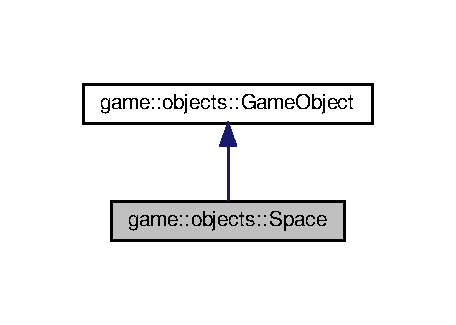
\includegraphics[width=219pt]{classgame_1_1objects_1_1Space__inherit__graph}
\end{center}
\end{figure}


Collaboration diagram for game\+:\+:objects\+:\+:Space\+:\nopagebreak
\begin{figure}[H]
\begin{center}
\leavevmode
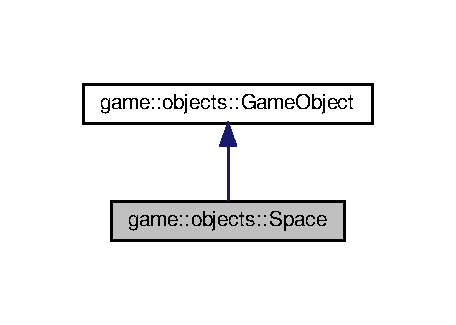
\includegraphics[width=219pt]{classgame_1_1objects_1_1Space__coll__graph}
\end{center}
\end{figure}
\subsection*{Public Member Functions}
\begin{DoxyCompactItemize}
\item 
\mbox{\Hypertarget{classgame_1_1objects_1_1Space_ac91aa556c22892e1e302744e0fd66873}\label{classgame_1_1objects_1_1Space_ac91aa556c22892e1e302744e0fd66873}} 
\hyperlink{classgame_1_1objects_1_1Space_ac91aa556c22892e1e302744e0fd66873}{Space} ()
\begin{DoxyCompactList}\small\item\em Construct a new \hyperlink{classgame_1_1objects_1_1Space}{Space} object with default values. \end{DoxyCompactList}\item 
bool \hyperlink{classgame_1_1objects_1_1Space_a3fe6ab73a208e58462a5883b398bc994}{Check} (char c)
\begin{DoxyCompactList}\small\item\em checks if the given character matches the \hyperlink{classgame_1_1objects_1_1Space}{Space}\textquotesingle{}s character \end{DoxyCompactList}\item 
char \hyperlink{classgame_1_1objects_1_1Space_a09d18080892a9c6d4d84ad2c81819a5e}{Letter} ()
\begin{DoxyCompactList}\small\item\em Letter Getter. \end{DoxyCompactList}\item 
void \hyperlink{classgame_1_1objects_1_1Space_a93ee0033d8184fac73533faca731fb08}{Letter} (char c)
\begin{DoxyCompactList}\small\item\em Letter Setter. \end{DoxyCompactList}\item 
\hyperlink{Validity_8h_acb8ce664e8a953fe8c27d7f0b37cbca4}{Validity} \hyperlink{classgame_1_1objects_1_1Space_a4d4114b0deca499cfe9ef6b5e3bdddc6}{Get\+Validity} ()
\begin{DoxyCompactList}\small\item\em Get the Validity field. \end{DoxyCompactList}\item 
void \hyperlink{classgame_1_1objects_1_1Space_a336887def7a71ac60ccfd2bb4a375df7}{Set\+Validity} (\hyperlink{Validity_8h_acb8ce664e8a953fe8c27d7f0b37cbca4}{Validity} v)
\begin{DoxyCompactList}\small\item\em Set the Validity field. \end{DoxyCompactList}\item 
std\+::string \hyperlink{classgame_1_1objects_1_1Space_a3df31a4e4a23a99baa7363df9a518705}{Name} () override
\begin{DoxyCompactList}\small\item\em Name getter. \end{DoxyCompactList}\item 
std\+::string \hyperlink{classgame_1_1objects_1_1Space_a1498390be3206f8c9e4e8f77bb939c31}{to\+\_\+string} () override
\begin{DoxyCompactList}\small\item\em coverts the letter to a string based on its Validity value \end{DoxyCompactList}\end{DoxyCompactItemize}


\subsection{Detailed Description}
\hyperlink{classgame_1_1objects_1_1Space}{Space} class for managing letters within the game \hyperlink{classgame_1_1objects_1_1Grid}{Grid}. 

\subsection{Member Function Documentation}
\mbox{\Hypertarget{classgame_1_1objects_1_1Space_a3fe6ab73a208e58462a5883b398bc994}\label{classgame_1_1objects_1_1Space_a3fe6ab73a208e58462a5883b398bc994}} 
\index{game\+::objects\+::\+Space@{game\+::objects\+::\+Space}!Check@{Check}}
\index{Check@{Check}!game\+::objects\+::\+Space@{game\+::objects\+::\+Space}}
\subsubsection{\texorpdfstring{Check()}{Check()}}
{\footnotesize\ttfamily bool game\+::objects\+::\+Space\+::\+Check (\begin{DoxyParamCaption}\item[{char}]{c }\end{DoxyParamCaption})}



checks if the given character matches the \hyperlink{classgame_1_1objects_1_1Space}{Space}\textquotesingle{}s character 


\begin{DoxyParams}{Parameters}
{\em c} & letter being checked \\
\hline
\end{DoxyParams}
\begin{DoxyReturn}{Returns}
true if c matches letter, false otherwise 
\end{DoxyReturn}
\mbox{\Hypertarget{classgame_1_1objects_1_1Space_a4d4114b0deca499cfe9ef6b5e3bdddc6}\label{classgame_1_1objects_1_1Space_a4d4114b0deca499cfe9ef6b5e3bdddc6}} 
\index{game\+::objects\+::\+Space@{game\+::objects\+::\+Space}!Get\+Validity@{Get\+Validity}}
\index{Get\+Validity@{Get\+Validity}!game\+::objects\+::\+Space@{game\+::objects\+::\+Space}}
\subsubsection{\texorpdfstring{Get\+Validity()}{GetValidity()}}
{\footnotesize\ttfamily \hyperlink{Validity_8h_acb8ce664e8a953fe8c27d7f0b37cbca4}{Validity} game\+::objects\+::\+Space\+::\+Get\+Validity (\begin{DoxyParamCaption}{ }\end{DoxyParamCaption})}



Get the Validity field. 

\begin{DoxyReturn}{Returns}
Validity 
\end{DoxyReturn}
\mbox{\Hypertarget{classgame_1_1objects_1_1Space_a09d18080892a9c6d4d84ad2c81819a5e}\label{classgame_1_1objects_1_1Space_a09d18080892a9c6d4d84ad2c81819a5e}} 
\index{game\+::objects\+::\+Space@{game\+::objects\+::\+Space}!Letter@{Letter}}
\index{Letter@{Letter}!game\+::objects\+::\+Space@{game\+::objects\+::\+Space}}
\subsubsection{\texorpdfstring{Letter()}{Letter()}\hspace{0.1cm}{\footnotesize\ttfamily [1/2]}}
{\footnotesize\ttfamily char game\+::objects\+::\+Space\+::\+Letter (\begin{DoxyParamCaption}{ }\end{DoxyParamCaption})}



Letter Getter. 

\begin{DoxyReturn}{Returns}
char letter 
\end{DoxyReturn}
\mbox{\Hypertarget{classgame_1_1objects_1_1Space_a93ee0033d8184fac73533faca731fb08}\label{classgame_1_1objects_1_1Space_a93ee0033d8184fac73533faca731fb08}} 
\index{game\+::objects\+::\+Space@{game\+::objects\+::\+Space}!Letter@{Letter}}
\index{Letter@{Letter}!game\+::objects\+::\+Space@{game\+::objects\+::\+Space}}
\subsubsection{\texorpdfstring{Letter()}{Letter()}\hspace{0.1cm}{\footnotesize\ttfamily [2/2]}}
{\footnotesize\ttfamily void game\+::objects\+::\+Space\+::\+Letter (\begin{DoxyParamCaption}\item[{char}]{c }\end{DoxyParamCaption})}



Letter Setter. 


\begin{DoxyParams}{Parameters}
{\em c} & new letter of the \hyperlink{classgame_1_1objects_1_1Space}{Space} \\
\hline
\end{DoxyParams}
\mbox{\Hypertarget{classgame_1_1objects_1_1Space_a3df31a4e4a23a99baa7363df9a518705}\label{classgame_1_1objects_1_1Space_a3df31a4e4a23a99baa7363df9a518705}} 
\index{game\+::objects\+::\+Space@{game\+::objects\+::\+Space}!Name@{Name}}
\index{Name@{Name}!game\+::objects\+::\+Space@{game\+::objects\+::\+Space}}
\subsubsection{\texorpdfstring{Name()}{Name()}}
{\footnotesize\ttfamily std\+::string game\+::objects\+::\+Space\+::\+Name (\begin{DoxyParamCaption}{ }\end{DoxyParamCaption})\hspace{0.3cm}{\ttfamily [override]}, {\ttfamily [virtual]}}



Name getter. 

\begin{DoxyReturn}{Returns}
std\+::string name of this object 
\end{DoxyReturn}


Implements \hyperlink{classgame_1_1objects_1_1GameObject_abc967efcbc66ec93c8592ad785aeb953}{game\+::objects\+::\+Game\+Object}.

\mbox{\Hypertarget{classgame_1_1objects_1_1Space_a336887def7a71ac60ccfd2bb4a375df7}\label{classgame_1_1objects_1_1Space_a336887def7a71ac60ccfd2bb4a375df7}} 
\index{game\+::objects\+::\+Space@{game\+::objects\+::\+Space}!Set\+Validity@{Set\+Validity}}
\index{Set\+Validity@{Set\+Validity}!game\+::objects\+::\+Space@{game\+::objects\+::\+Space}}
\subsubsection{\texorpdfstring{Set\+Validity()}{SetValidity()}}
{\footnotesize\ttfamily void game\+::objects\+::\+Space\+::\+Set\+Validity (\begin{DoxyParamCaption}\item[{\hyperlink{Validity_8h_acb8ce664e8a953fe8c27d7f0b37cbca4}{Validity}}]{v }\end{DoxyParamCaption})}



Set the Validity field. 


\begin{DoxyParams}{Parameters}
{\em v} & new Validity value \\
\hline
\end{DoxyParams}
\mbox{\Hypertarget{classgame_1_1objects_1_1Space_a1498390be3206f8c9e4e8f77bb939c31}\label{classgame_1_1objects_1_1Space_a1498390be3206f8c9e4e8f77bb939c31}} 
\index{game\+::objects\+::\+Space@{game\+::objects\+::\+Space}!to\+\_\+string@{to\+\_\+string}}
\index{to\+\_\+string@{to\+\_\+string}!game\+::objects\+::\+Space@{game\+::objects\+::\+Space}}
\subsubsection{\texorpdfstring{to\+\_\+string()}{to\_string()}}
{\footnotesize\ttfamily std\+::string game\+::objects\+::\+Space\+::to\+\_\+string (\begin{DoxyParamCaption}{ }\end{DoxyParamCaption})\hspace{0.3cm}{\ttfamily [override]}, {\ttfamily [virtual]}}



coverts the letter to a string based on its Validity value 

\begin{DoxyReturn}{Returns}
std\+::string wrapped letter 
\end{DoxyReturn}


Implements \hyperlink{classgame_1_1objects_1_1GameObject_a59faf4c33c2c0d8a9d52a26029d1488f}{game\+::objects\+::\+Game\+Object}.



The documentation for this class was generated from the following file\+:\begin{DoxyCompactItemize}
\item 
inc/game/objects/Space.\+h\end{DoxyCompactItemize}

\chapter{File Documentation}
\hypertarget{Color_8h}{}\section{inc/game/\+Color.h File Reference}
\label{Color_8h}\index{inc/game/\+Color.\+h@{inc/game/\+Color.\+h}}
{\ttfamily \#include $<$string$>$}\newline
Include dependency graph for Color.\+h\+:\nopagebreak
\begin{figure}[H]
\begin{center}
\leavevmode
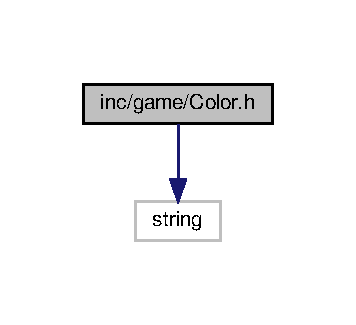
\includegraphics[width=171pt]{Color_8h__incl}
\end{center}
\end{figure}
\subsection*{Enumerations}
\begin{DoxyCompactItemize}
\item 
\mbox{\Hypertarget{Color_8h_a24bd400aac9e8042c9d717391e45655a}\label{Color_8h_a24bd400aac9e8042c9d717391e45655a}} 
enum \hyperlink{Color_8h_a24bd400aac9e8042c9d717391e45655a}{game\+::color\+::\+Code} \{ \newline
{\bfseries F\+G\+\_\+\+R\+ED} = 31, 
{\bfseries F\+G\+\_\+\+G\+R\+E\+EN} = 32, 
{\bfseries F\+G\+\_\+\+B\+L\+UE} = 34, 
{\bfseries F\+G\+\_\+\+D\+E\+F\+A\+U\+LT} = 39, 
\newline
{\bfseries B\+G\+\_\+\+R\+ED} = 41, 
{\bfseries B\+G\+\_\+\+G\+R\+E\+EN} = 42, 
{\bfseries B\+G\+\_\+\+B\+L\+UE} = 44, 
{\bfseries B\+G\+\_\+\+D\+E\+F\+A\+U\+LT} = 49
 \}\begin{DoxyCompactList}\small\item\em Color code enumeration for changing color of text printed to terminal. \end{DoxyCompactList}
\end{DoxyCompactItemize}
\subsection*{Functions}
\begin{DoxyCompactItemize}
\item 
std\+::string \hyperlink{Color_8h_af6672ccde6549bd1741d68ed0b7e0f42}{game\+::color\+::wrap} (const std\+::string \&str, Code c)
\begin{DoxyCompactList}\small\item\em wraps the given string in the encoding of the specified color code. When printed to terminal, string will appear in the specified color \end{DoxyCompactList}\end{DoxyCompactItemize}


\subsection{Function Documentation}
\mbox{\Hypertarget{Color_8h_file_af6672ccde6549bd1741d68ed0b7e0f42}\label{Color_8h_file_af6672ccde6549bd1741d68ed0b7e0f42}} 
\index{Color.\+h@{Color.\+h}!wrap@{wrap}}
\index{wrap@{wrap}!Color.\+h@{Color.\+h}}
\subsubsection{\texorpdfstring{wrap()}{wrap()}}
{\footnotesize\ttfamily std\+::string game\+::color\+::wrap (\begin{DoxyParamCaption}\item[{const std\+::string \&}]{str,  }\item[{\hyperlink{Color_8h_a24bd400aac9e8042c9d717391e45655a}{Code}}]{c }\end{DoxyParamCaption})\hspace{0.3cm}{\ttfamily [inline]}}



wraps the given string in the encoding of the specified color code. When printed to terminal, string will appear in the specified color 


\begin{DoxyParams}{Parameters}
{\em str} & string that will be wrapped in color-\/encodings \\
\hline
{\em c} & desired color code \\
\hline
\end{DoxyParams}
\begin{DoxyReturn}{Returns}
std\+::string wrapped string 
\end{DoxyReturn}

\hypertarget{Dictionary_8h}{}\section{inc/game/\+Dictionary.h File Reference}
\label{Dictionary_8h}\index{inc/game/\+Dictionary.\+h@{inc/game/\+Dictionary.\+h}}
{\ttfamily \#include $<$set$>$}\newline
{\ttfamily \#include $<$string$>$}\newline
Include dependency graph for Dictionary.\+h\+:\nopagebreak
\begin{figure}[H]
\begin{center}
\leavevmode
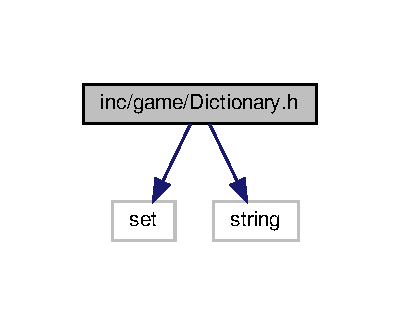
\includegraphics[width=192pt]{Dictionary_8h__incl}
\end{center}
\end{figure}
This graph shows which files directly or indirectly include this file\+:\nopagebreak
\begin{figure}[H]
\begin{center}
\leavevmode
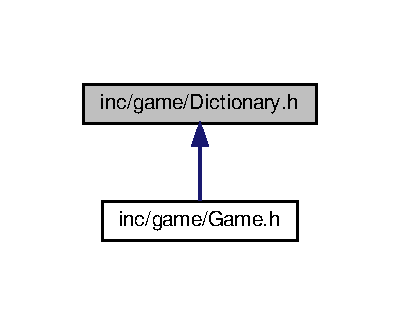
\includegraphics[width=192pt]{Dictionary_8h__dep__incl}
\end{center}
\end{figure}
\subsection*{Classes}
\begin{DoxyCompactItemize}
\item 
class \hyperlink{classgame_1_1Dictionary}{game\+::\+Dictionary}
\begin{DoxyCompactList}\small\item\em \hyperlink{classgame_1_1Dictionary}{Dictionary} class for handling acceptable words for the game. Loads words from system file. \end{DoxyCompactList}\end{DoxyCompactItemize}

\hypertarget{Validity_8h}{}\section{inc/game/\+Validity.h File Reference}
\label{Validity_8h}\index{inc/game/\+Validity.\+h@{inc/game/\+Validity.\+h}}
{\ttfamily \#include $<$stdexcept$>$}\newline
{\ttfamily \#include $<$string$>$}\newline
Include dependency graph for Validity.\+h\+:
\nopagebreak
\begin{figure}[H]
\begin{center}
\leavevmode
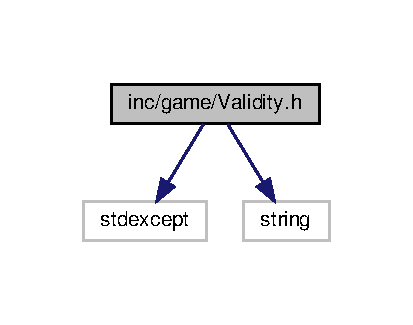
\includegraphics[width=198pt]{Validity_8h__incl}
\end{center}
\end{figure}
This graph shows which files directly or indirectly include this file\+:
\nopagebreak
\begin{figure}[H]
\begin{center}
\leavevmode
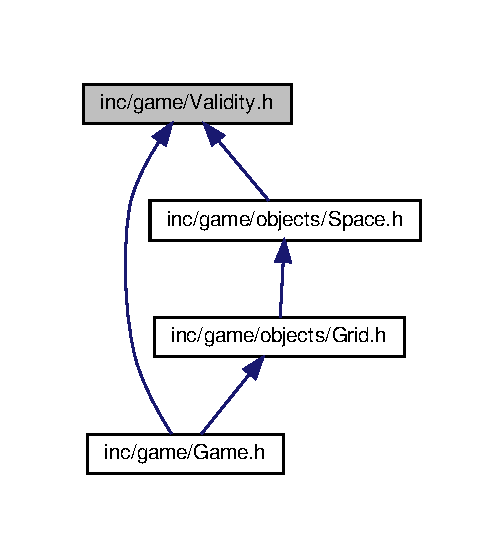
\includegraphics[width=242pt]{Validity_8h__dep__incl}
\end{center}
\end{figure}
\subsection*{Enumerations}
\begin{DoxyCompactItemize}
\item 
\mbox{\Hypertarget{Validity_8h_acb8ce664e8a953fe8c27d7f0b37cbca4}\label{Validity_8h_acb8ce664e8a953fe8c27d7f0b37cbca4}} 
enum \hyperlink{Validity_8h_acb8ce664e8a953fe8c27d7f0b37cbca4}{game\+::\+Validity} \{ {\bfseries E\+M\+P\+TY} = 0, 
{\bfseries I\+N\+V\+A\+L\+ID} = 1, 
{\bfseries C\+L\+O\+SE} = 2, 
{\bfseries C\+O\+R\+R\+E\+CT} = 3
 \}\begin{DoxyCompactList}\small\item\em enumeration for decided how close a guessed letter is to the truth \end{DoxyCompactList}
\end{DoxyCompactItemize}
\subsection*{Functions}
\begin{DoxyCompactItemize}
\item 
std\+::string \hyperlink{Validity_8h_ae94e241b67d39183fe443e95cb2c3a7b}{game\+::to\+\_\+string} (Validity v)
\begin{DoxyCompactList}\small\item\em to string function for Validity enumeration \end{DoxyCompactList}\item 
Validity \hyperlink{Validity_8h_a27f760049e18d6c9fa017073934d5b35}{game\+::from\+\_\+string} (const std\+::string \&s)
\begin{DoxyCompactList}\small\item\em from\+\_\+string function to convert a specfic set of strings to Validity enum values \end{DoxyCompactList}\end{DoxyCompactItemize}


\subsection{Function Documentation}
\mbox{\Hypertarget{Validity_8h_file_a27f760049e18d6c9fa017073934d5b35}\label{Validity_8h_file_a27f760049e18d6c9fa017073934d5b35}} 
\index{Validity.\+h@{Validity.\+h}!from\+\_\+string@{from\+\_\+string}}
\index{from\+\_\+string@{from\+\_\+string}!Validity.\+h@{Validity.\+h}}
\subsubsection{\texorpdfstring{from\+\_\+string()}{from\_string()}}
{\footnotesize\ttfamily Validity game\+::from\+\_\+string (\begin{DoxyParamCaption}\item[{const std\+::string \&}]{s }\end{DoxyParamCaption})\hspace{0.3cm}{\ttfamily [inline]}}



from\+\_\+string function to convert a specfic set of strings to Validity enum values 


\begin{DoxyParams}{Parameters}
{\em s} & string that will be converted to equivalent Validity value \\
\hline
\end{DoxyParams}
\begin{DoxyReturn}{Returns}
Validity equivalent to the given string 
\end{DoxyReturn}

\begin{DoxyExceptions}{Exceptions}
{\em std\+::invalid\+\_\+argument} & if the string does not match any names of the Validity enums \\
\hline
\end{DoxyExceptions}
\mbox{\Hypertarget{Validity_8h_file_ae94e241b67d39183fe443e95cb2c3a7b}\label{Validity_8h_file_ae94e241b67d39183fe443e95cb2c3a7b}} 
\index{Validity.\+h@{Validity.\+h}!to\+\_\+string@{to\+\_\+string}}
\index{to\+\_\+string@{to\+\_\+string}!Validity.\+h@{Validity.\+h}}
\subsubsection{\texorpdfstring{to\+\_\+string()}{to\_string()}}
{\footnotesize\ttfamily std\+::string game\+::to\+\_\+string (\begin{DoxyParamCaption}\item[{\hyperlink{Validity_8h_acb8ce664e8a953fe8c27d7f0b37cbca4}{Validity}}]{v }\end{DoxyParamCaption})\hspace{0.3cm}{\ttfamily [inline]}}



to string function for Validity enumeration 


\begin{DoxyParams}{Parameters}
{\em v} & enum value being converted to a std\+::string \\
\hline
\end{DoxyParams}
\begin{DoxyReturn}{Returns}
std\+::string name of the enum 
\end{DoxyReturn}

\begin{DoxyExceptions}{Exceptions}
{\em std\+::invalid\+\_\+argument} & if bad enum value is given \\
\hline
\end{DoxyExceptions}

%--- End generated contents ---

% Index
\backmatter
\newpage
\phantomsection
\clearemptydoublepage
\addcontentsline{toc}{chapter}{Index}
\printindex

\end{document}
